\section{基于BC-TD3的制导参数优化}
本节将开发基于BC-TD3的制导参数优化框架，以解决问题3。首先，根据闭环制导定律\eqref{eq:66}的结构，连续时间参数优化问题通过单打靶法转录为有限维非线性规划（NLP）问题，并在随机抽样初始条件下离线生成满足最小规避距离和目标到达精度约束的专家轨迹。然后构建BC-TD3网络：actor通过专家演示的行为克隆预训练，随后通过双延迟深度确定性策略梯度（TD3）微调，以进一步提升泛化和闭环性能。

\subsection{专家轨迹生成}
假设NCV仿真初始位置与目标重合，即为坐标系OXYZ原点。由几何关系知，NCV速度前置角

\begin{equation}
\label{eq:67}
\left\{ {\begin{array}{*{20}{l}}
  {{\eta _{{y_{Di}}}} = {\theta _{Di}} - {q_{yi}}} \\ 
  {{\eta _{{z_{Di}}}} = {\psi _{{V_{Di}}}} - {q_{zi}}} 
\end{array},{\text{ }}i = 1,2} \right.
\end{equation}
规避者相对于第i枚NCV的速度前置角

\begin{equation}
\label{eq:68}
\left\{ {\begin{array}{*{20}{l}}
  {{\eta _{yAi}} = {\theta _A} + {q_{yi}}} \\ 
  {{\eta _{zAi}} = {\psi _{{V_A}}} - {q_{zi}} - \pi } 
\end{array}} \right.
\end{equation}
综合考虑影响规避效能的主要因素，设规避方与第i枚NCV相对位置的初始角度状态为${X_i} = [{q_{yi0}},{q_{zi0}},{\eta _{yAi0}},{\eta _{zAi0}},{\eta _{yDi0}},{\eta _{zDi0}}](i = 1,2)$。考虑到实际中同时出现的NCV与规避方的初始距离差通常不会过大，假定当规避方与某一NCV进入规避状态时，两枚NCV与规避方的距离差小于3km。设随机变量$\beta  \in [ - 1.5,1.5]{\text{km}}$为调节变量，${r_{AD{\text{0}}}}$为中值，并满足${r_{AD10}} = {r_{AD0}} + \beta $, ${r_{AD20}} = {r_{AD0}} - \beta $。由此，以14维初始状态向量$X = {[{X_1},{X_2},{r_{AD0}},\beta ]^T}$作为全程飞行的初始状态，并以制导参数向量${\mathbf{p}} = {[w,{\kern 1pt} \gamma ,{\kern 1pt} {w_T},{\kern 1pt} {w_E}]^T}$为待定参数，可在打靶法和强化学习训练中进行求解.
单次打靶法（single shooting）是求解连续时间最优控制问题的一类直接转录方法，实现简便，且与标准NLP求解器兼容性好。与在密集节点上同时离散化状态与控制的配点法不同，单次打靶法仅对决策变量进行参数化，并通过系统动力学前向积分恢复轨迹，从而将无穷维最优控制问题转化为有限维参数优化问题。

在交会区间$[{t_0},{t_f}]$上，待决策的制导参数向量${\mathbf{p}} = {[w,{\kern 1pt} \gamma ,{\kern 1pt} {w_T},{\kern 1pt} {w_E}]^T}$由K段分段常值表示：

\begin{equation}
\label{eq:69}
{\mathbf{p}}(t) = {{\mathbf{p}}_k},\quad t \in [{t_{k - 1}},{\kern 1pt} {t_k}),\quad k = 1, \ldots ,K
\end{equation}
其中K=10，${\mathbf{p}} = {[w,{\kern 1pt} \gamma ,{\kern 1pt} {w_T},{\kern 1pt} {w_E}]^T}$，分段边界均匀划分。由于真正在目标函数中发挥作用的是权重比值而非绝对大小，因此令总规避权重固定为${w_k} = w = {10^4}$，从而实际决策变量为各段的$[{\gamma _k},{\kern 1pt} {w_{T,k}},{\kern 1pt} {w_{E,k}}]$。期望规避距离为一固定值，这里不妨假定为${d^*} = 20{\kern 1pt} {\text{m}}$。

给定候选参数序列$\{ {{\mathbf{p}}_k}\} _{k = 1}^K$后，对交会运动学\eqref{eq:1}-\eqref{eq:5}采用四阶龙格—库塔（RK4）前向积分，步长$\Delta t = 0.1{\kern 1pt} {\text{s}}$：

\begin{equation}
\label{eq:70}
X({t_{n + 1}}) = X({t_n}) + \frac{{\Delta t}}{6}({k_1} + 2{k_2} + 2{k_3} + {k_4})
\end{equation}
其中$X$表示完整系统状态，${k_1}, \ldots ,{k_4}$为在当前段参数下、由闭环制导律\eqref{eq:66}计算得到的RK4增量。NLP目标按性能指标\eqref{eq:23}构造：

\begin{equation}
\label{eq:71}
\mathop {\min }\limits_{\{ {{\mathbf{p}}_k}\} _{k = 1}^K} \mathcal{J} = {s_w}\sum\limits_{i = 1}^2 {{{\left[ {d_i^{{\text{actual}}} - {d_i}} \right]}^2}}  + {s_{{w_E}}}\int_{{t_0}}^{{t_f}} {{\mathbf{u}}_A^T{{\mathbf{u}}_A}d\tau }  + {s_{{w_T}}}{\left\| {{r_{AT}}({t_f})} \right\|^2}
\end{equation}
其中${s_w} = 2 \times {10^3},{s_{{w_E}}} = 55,{s_{{w_T}}} = 22$为固定缩放系数，$d_i^{{\text{actual}}}$为相对NCV D\_i的实际最小接近距离。所得的NLP通过IPOPT采用L-BFGS黑森近似求解。

单打靶法求解得到的轨迹作为后续BC-TD3训练的专家示范。专家数据集记为${\mathcal{D}_{{\text{expert}}}} = \{ {\zeta ^{(1)}},{\kern 1pt} {\zeta ^{(2)}},{\kern 1pt}  \ldots ,{\kern 1pt} {\zeta ^{({N_{{\text{expert}}}})}}\} $，其中每条轨迹${\zeta ^{(\ell )}} = \{ ({\mathbf{s}}_n^{(\ell )},{\kern 1pt} {\mathbf{a}}_n^{(\ell )})\} _{n = 1}^{{N_\ell }}$由从轨迹提取的${N_t}$个状态—动作对组成。共在14维初始状态空间上通过拉丁超立方抽样抽取${N_{{\text{expert}}}} = 2400$组初始条件，约得到$8{\text{ - }}15 \times {10^4}$对专家示范状态—动作对样本。

\subsection{BC-TD3算法网络构建}
\subsubsection{状态空间、动作空间与奖励函数}
状态空间（13 维相对交会状态）：

\begin{equation}
\label{eq:72}
{\mathbf{s}}(t) = {[\underbrace {{r_{A{D_1}}},{\kern 1pt} {{\dot r}_{A{D_1}}},{\kern 1pt} {q_{{y_1}}},{\kern 1pt} {q_{{z_1}}}}_{{\text{NCV 1}}},\;\underbrace {{r_{A{D_2}}},{\kern 1pt} {{\dot r}_{A{D_2}}},{\kern 1pt} {q_{{y_2}}},{\kern 1pt} {q_{{z_2}}}}_{{\text{NCV 2}}},\;\underbrace {{r_{AT}},{\kern 1pt} {q_{{y_T}}},{\kern 1pt} {q_{{z_T}}}}_{{\text{Target}}},\;\underbrace {{V_A},{\kern 1pt} \bar{t}_{go}}_{{\text{Evader}}}]^T} \in {\mathbb{R}^{13}}
\end{equation}
其中$\bar{t}_{go} = \min ({t_{go,1}},{t_{go,2}})$为两枚NCV中的最小剩余飞行时间。该状态表征规避方与两枚NCV及目标的相对几何与运动学，以支撑制导律参数决策。

动作空间（3维制导参数向量）：

\begin{equation}
\label{eq:73}
{\mathbf{a}}(t) = {[\frac{w}{{{w_E}}},{\kern 1pt} \frac{{{w_T}}}{{{w_E}}},\gamma ]^T} \in {\mathbb{R}^3}
\end{equation}
其中，$w$表示两枚NCV规避项权重${w_1}$,${w_2}$之和，$\gamma $用于表征${w_1}$,${w_2}$间大小关系，${w_E}$表示能量消耗项权重；这些参数详细含义可参见第2节末尾。

奖励函数设计：奖励由规避阶段的逐步过程奖励，加上第3阶段PN积分前滚后结算的终端奖励构成。过程奖励为：

\begin{equation}
\label{eq:74}
\left\{
\begin{aligned}
& {R_1} = 0.05{\log _{10}}(\min ({r_{AD1}},{d^*}) - 5),if{\text{ }}{r_{AD1,\min }} \geqslant 6{\text{m }}else{\text{ }}0 \\
& {R_2} = 0.05{\log _{10}}(\min ({r_{AD2}},{d^*}) - 5),if{\text{ }}{r_{AD2,\min }} \geqslant 6{\text{m }}else{\text{ }}0
\end{aligned}
\right.
\end{equation}
其中，R1、R2分别为规避两枚NCV的过程奖励项，${r_{ADi,\min }} = \min {r_{ADi}}(t)$为整段交会中相对NCV ${D_i}$的最小接近距离。

终端奖励为

\begin{equation}
\label{eq:75}
\left\{
\begin{aligned}
& {R_T} = \frac{{80}}{{5 + {r_{AT,end}}}} \\
& {R_{bonus}} = 100,{\text{ }}if{\text{ }}{r_{AT,end}} \leqslant 10{\text{m }}else{\text{ }}0 \\
& {R_{penalty}} =  - 50,{\text{ }}if{\text{ min(}}{r_{AD1,\min }},{r_{AD2,\min }}{\text{)}} \leqslant 6{\text{m }}else{\text{ }}0
\end{aligned}
\right.
\end{equation}
其中，${r_{AT,end}}$为由第3阶段PN前滚得到的对目标末端到达误差，RT为根据实际得到的终端目标精度给出的目标到达精度项奖励。${R_{bonus}}$为同时完成规避和目标到达任务后给出的专门奖励，${R_{penalty}}$为规避失败后给出的专门惩罚项。

\subsubsection{网络架构}
BC-TD3框架采用两阶段训练范式：行为克隆（BC）预训练，再经TD3强化学习微调。两阶段均完全离线进行。

Actor 网络 ${\pi _\phi }({\mathbf{s}})$：将13维状态映射为4维动作：

\begin{equation}
\label{eq:76}
{\pi _\phi }({\mathbf{s}}) = {{\mathbf{a}}_{\max }} \cdot \tanh ({{\mathbf{W}}_3}{\kern 1pt} {\text{ReLU}}({{\mathbf{W}}_2}{\kern 1pt} {\text{ReLU}}({{\mathbf{W}}_1}{\mathbf{s}} + {{\mathbf{b}}_1}) + {{\mathbf{b}}_2}) + {{\mathbf{b}}_3})
\end{equation}
隐层为[256, 256]，ReLU激活，输出层为tanh以实现有界动作。

双Critic网络${Q_{{\psi _1}}}({\mathbf{s}},{\mathbf{a}}),{Q_{{\psi _2}}}({\mathbf{s}},{\mathbf{a}})$：各自将拼接后的$({\mathbf{s}},{\mathbf{a}})$映射为标量Q值。

\begin{equation}
\label{eq:77}
{Q_{{\psi _j}}}({\mathbf{s}},{\mathbf{a}}) = {\mathbf{W}}_3^{(j)}{\kern 1pt} {\text{ReLU}}({\mathbf{W}}_2^{(j)}{\kern 1pt} {\text{ReLU}}({\mathbf{W}}_1^{(j)}[{\mathbf{s}};{\kern 1pt} {\mathbf{a}}] + {\mathbf{b}}_1^{(j)}) + {\mathbf{b}}_2^{(j)}) + b_3^{(j)},\quad j = 1,2
\end{equation}
隐层为[256, 256]，线性输出。目标网络 \(\pi_{\phi'}\)、\(Q_{\psi_1'}\)、\(Q_{\psi_2'}\)以软拷贝方式维护，以保证训练稳定。

对BC预训练，Actor网络首先在专家数据集$({\mathcal{D}_{{\text{expert}}}} = \{ ({{\mathbf{s}}_n},{{\mathbf{a}}_n})\} _{n = 1}^{{N_{{\text{expert}}}}})$上以有监督行为克隆预训练：

\begin{equation}
\label{eq:78}
{\mathcal{L}_{{\text{BC}}}}(\phi ) = \frac{1}{N}\sum\limits_{n = 1}^N {{{\left\| {{\pi _\phi }({{\mathbf{s}}_n}) - {{\mathbf{a}}_n}} \right\|}^2}} 
\end{equation}
预训练得到的Actor参数${\phi _{{\text{BC}}}}$为TD3微调提供热启动。此外，专家状态–动作对预填入经验回放缓冲区$\mathcal{R}$，使TD3早期训练即可受益于高质量示范。

TD3的裁剪双Q与延迟策略更新可缓解DDPG的Q值过估计与策略振荡，从而在多约束任务中收敛更稳健。TD3相对DDPG的三项关键机制如下：

(1)裁剪双Q。目标值取两个Critic估计的最小值，以抑制过估计偏差：

\begin{equation}
\label{eq:79}
{y_n} = {r_n} + \gamma {\kern 1pt} {\min _{j = 1,2}}{Q_{{\psi _{j'}}}}({{\mathbf{s}}_{n + 1}},{\kern 1pt} {\tilde{\mathbf{a}}_{n + 1}})
\end{equation}
其中目标动作包含目标策略平滑：

\begin{equation}
\label{eq:80}
{\tilde{\mathbf{a}}_{n + 1}} = {\pi _{\phi '}}({{\mathbf{s}}_{n + 1}}) + {\boldsymbol{\epsilon }},\quad {\boldsymbol{\epsilon }} \sim {\text{clip}}\left( {\mathcal{N}({\mathbf{0}},\sigma _p^2{\mathbf{I}}), - c,c} \right)
\end{equation}
Critic损失：

\begin{equation}
\label{eq:81}
{\mathcal{L}_{{\text{Critic}}}}({\psi _j}) = \frac{1}{N}\sum\limits_{n = 1}^N ( {y_n} - {Q_{{\psi _j}}}({{\mathbf{s}}_n},{{\mathbf{a}}_n}){)^2},\quad j = 1,2
\end{equation}
(2)延迟策略更新。Actor每d步更新一次（通常d=2），而非每步更新，以降低快速变化的Critic目标与策略更新之间的耦合：

\begin{equation}
\label{eq:82}
{\nabla _\phi }J = \frac{1}{N}\sum\limits_{n = 1}^N {{\nabla _{\mathbf{a}}}} {Q_{{\psi _1}}}({{\mathbf{s}}_n},{\mathbf{a}}){|_{{\mathbf{a}} = {\pi _\phi }({{\mathbf{s}}_n})}} \cdot {\nabla _\phi }{\pi _\phi }({{\mathbf{s}}_n})
\end{equation}
(3)目标网络软更新（与Actor相同的延迟频率执行）：

\begin{equation}
\label{eq:83}
\phi ' \leftarrow \tau \phi  + (1 - \tau )\phi ',\qquad {\psi _{j'}} \leftarrow \tau {\psi _j} + (1 - \tau ){\psi _{j'}}
\end{equation}
其中$\tau  \ll 1$（例如$\tau  = 0.005$）。

微调阶段的探索噪声. 环境交互时在Actor 输出上叠加高斯噪声：

\begin{equation}
\label{eq:84}
{{\mathbf{a}}_n} = {\pi _\phi }({{\mathbf{s}}_n}) + {{\mathbf{\eta }}_n},\quad {{\mathbf{\eta }}_n}\sim \mathcal{N}({\mathbf{0}},{\kern 1pt} \sigma _e^2{\mathbf{I}})
\end{equation}
其中${\sigma _e}$随训练回合衰减，以实现由探索向利用的过渡。

BC-TD3整体网络架构如下图~\ref{fig:bctd3-arch}所示：

\begin{figure}[htbp]
\centering
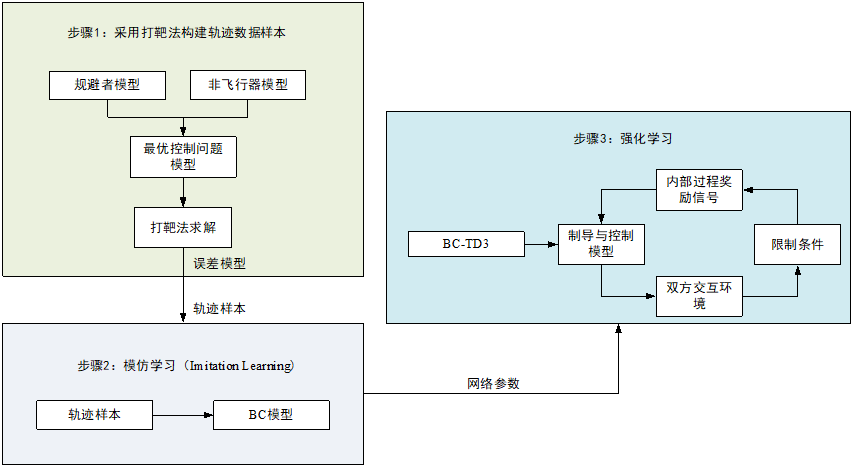
\includegraphics[width=0.82\linewidth]{fig02}
\caption{BC-TD3网络架构图}
\label{fig:bctd3-arch}
\end{figure}
BC-TD3与TD3网络训练超参数如下表~\ref{tab:hyperparams}所示：

\begin{table}[htbp]
\centering
\caption{TD3与BC-TD3训练超参数}
\label{tab:hyperparams}
\small
\begin{tabularx}{\linewidth}{lXX}
\toprule
超参数 & TD3 & BC-TD3 \\
\midrule
总训练步数 & 300 000 & 300 000 \\
学习率 & 1$\times$$10^{-4}$ & 1$\times$$10^{-4}$ \\
批次大小 & 256 & 256 \\
折扣因子 $\gamma$ & 0.99 & 0.99 \\
软更新系数 $\tau$ & 0.005 & 0.005 \\
经验回放容量 & 300 000 & 300 000 \\
开始更新步数 & 1 000 & 0 \\
训练频率 & 1 步 & 1 步 \\
策略延迟更新 & 3 & 3 \\
网络结构 & [256, 256] & [256, 256] \\
探索噪声 $\sigma$ & 0.1 & 0.1 \\
目标策略噪声 & 0.2 & 0.2 \\
目标噪声裁剪 & 0.5 & 0.5 \\
梯度裁剪 & ±10 & ±10 \\
BC 预填充比例 & — & 0.33 \\
BC 正则初始系数 $\lambda$$_0$ & — & 1.0 \\
BC 衰减步数 & — & 200 000 \\
\bottomrule
\end{tabularx}
\end{table}
\FloatBarrier
\subsubsection{BC-TD3算法网络训练}
完整离线训练流程如下：

\begin{algorithm}[H]
\caption{面向制导参数优化的 BC-TD3 离线训练}
\label{alg:bctd3}
{\footnotesize
\raggedright
输入：专家数据集 \(\mathcal{D}_{\text{expert}}\)，交会仿真器 \(\text{Env}\)\\
输出：训练后的 Actor \(\pi_\phi\)\\
// 阶段 1：BC 预训练\\
1: 以随机权重初始化 Actor \(\pi_\phi\)\\
2: for epoch = 1 to \(E_{\text{BC}}\) do\\
3:   从 \(\mathcal{D}_{\text{expert}}\) 采样小批量 \(\{(\boldsymbol{s}_n, \boldsymbol{a}_n)\}\)\\
4:   通过最小化 \(\mathcal{L}_{\text{BC}}\) 更新 \(\phi\)（式 \ref{eq:78}）\\
5: end for\\
6: 用 \(\mathcal{D}_{\text{expert}}\) 预填回放缓冲区 \(\mathcal{R}\)\\
// 阶段 2：TD3 微调\\
7: 初始化 Critic \(\psi_1, \psi_2\)，目标网络 \(\phi' \leftarrow \phi\)，\(\psi_j' \leftarrow \psi_j\)\\
8: for episode = 1 to \(E_{\text{TD3}}\) do\\
9:   将 Env 重置为随机初始条件 \(\boldsymbol{s}_0\)\\
10:  for \(n = 0, 1, 2, \ldots\) do\\
11:    \(\boldsymbol{a}_n = \pi_\phi(\boldsymbol{s}_n) + \boldsymbol{\eta}_n\)                    // 式 \ref{eq:84}\\
12:    在 Env 中执行 \(\boldsymbol{a}_n\) \(\to\) 由式 \eqref{eq:66} 得到 \(\boldsymbol{u}_A^*(t)\)\\
13:    观测 \(\boldsymbol{s}_{n+1}, r_n\)（式 \ref{eq:74}--\ref{eq:75}）\\
14:    将 \((\boldsymbol{s}_n, \boldsymbol{a}_n, r_n, \boldsymbol{s}_{n+1})\) 存入 \(\mathcal{R}\)\\
15:    从 \(\mathcal{R}\) 采样 \(N\) 条转移的小批量\\
16:    计算目标 \(y_n\)（式 \ref{eq:79}--\ref{eq:80}）\\
17:    通过最小化 \(\mathcal{L}_{\text{Critic}}\) 更新 Critic \(\psi_1, \psi_2\)（式 \ref{eq:81}）\\
18:    if \(n \mod d = 0\) then                                           // 延迟更新\\
19:      通过策略梯度更新 Actor \(\phi\)（式 \ref{eq:82}）\\
20:      软更新目标网络：\(\phi', \psi_j'\)（式 \ref{eq:83}）\\
21:    end if\\
22:  end for\\
23: end for\\
// 部署（在线推理）\\
24: return \(\pi_\phi\) — 每个制导周期：\(\boldsymbol{a} = \pi_\phi(\boldsymbol{s})\)，将 \(\boldsymbol{a}\) 与辨识矩阵送入式 \eqref{eq:66}
}
\end{algorithm}
